\section{Simulation Studies}
\label{sec:simu}

This section presents simulation studies to examine the empirical performance of the proposed model selection frameworks under different noise settings. 
In Section \ref{subsec:study1} and \ref{subsec:STLSQ}, we investigate the Bayesian Razor method and STLSQ algorithm for polynomial regression models with noise only in the response variable. 
In Section \ref{subsec:study2}, we evaluate the STLSQ-ODR procedure for polynomial regression models with noise in both predictors and responses, considering Gaussian, Student-t, and correlated noise structures. Across all experiments, we generate synthetic datasets from polynomial ground truth models, systematically vary the noise levels, and assess model recovery accuracy in terms of posterior probabilities and sparse coefficient estimation.

\subsection{Study 1: Bayesian Razor Method Evidence}
\label{subsec:study1}

This subsection conducts the empirical performance of Bayesian Razor for a polynomial regression model with added noise in the response variable. 
Specifically, we consider a univariate polynomial regression setting, where the true data-generating function is a cubic polynomial given by $y = 3 - 2x + x^3$ with additive Gaussian noise $\varepsilon_i \sim \mathcal{N}(0, \sigma^2)$ in $y$, where $\sigma = 0.1, 0.3,0.5$. We use $n=1000$ evenly spaced input points over $[-1, 1]$ to simulate a low-data regime.

To explore the performance of Bayesian model selection under limited data, we evaluate all $2^4 - 1 = 15$ non-empty subsets of candidate polynomial basis functions ${1, x, x^2, x^3}$. For each subset, we compute the MAP estimate of the regression coefficients under a zero-mean Gaussian prior with unit variance, and calculate the marginal likelihood (evidence) assuming a fixed likelihood precision.


The posterior probability of each model is computed by normalising its marginal likelihood across all models. We then compare these models in terms of both their posterior probability and coefficient estimates, ultimately identifying the model with the highest posterior probability. 

\begin{figure}[htbp]
\centering
\begin{minipage}{0.47\textwidth}
    \centering
    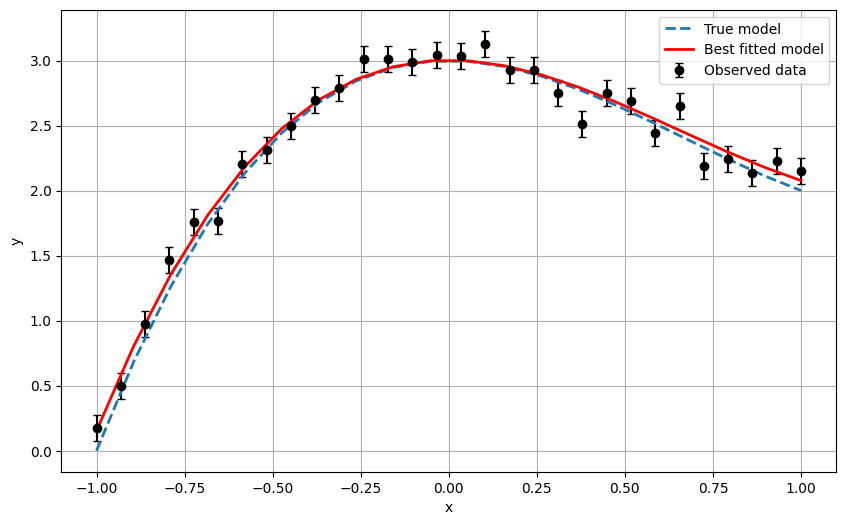
\includegraphics[width=\linewidth]{MSc_Statistics_Research_Report_Template/images/n=30, sigma=0.1.png}
    \subcaption{$n=30$, $\sigma=0.1$}
\end{minipage}
\begin{minipage}{0.47\textwidth}
    \centering
    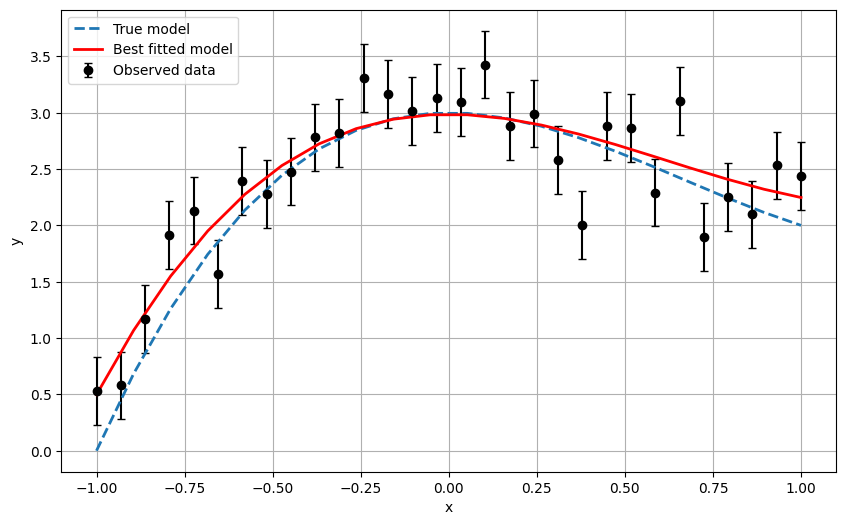
\includegraphics[width=\linewidth]{MSc_Statistics_Research_Report_Template/images/n=30, sigma=0.3.png}
    \subcaption{$n=30$, $\sigma=0.3$}
\end{minipage}
\begin{minipage}{0.47\textwidth}
    \centering
    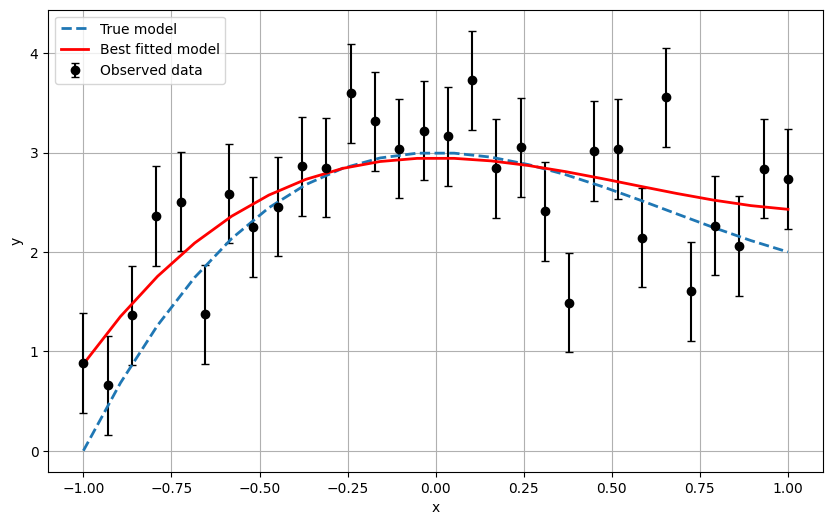
\includegraphics[width=\linewidth]{MSc_Statistics_Research_Report_Template/images/n=30, sigma=0.5.png} 
    \subcaption{$n=30$, $\sigma=0.5$}
\end{minipage}
\begin{minipage}{0.47\textwidth}
    \centering
    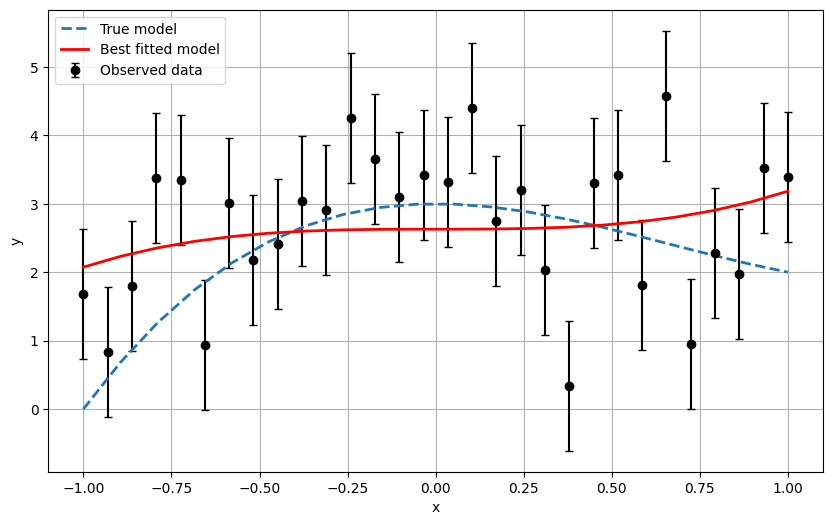
\includegraphics[width=\linewidth]{MSc_Statistics_Research_Report_Template/images/n=30, sigma=0.95.png}
    \subcaption{$n=30$, $\sigma=0.95$}
\end{minipage}
\caption{Comparison of the true model, best fitted model, and observed data with different error bars.}
\label{fig:n=30}
\end{figure}

Table \ref{tab:Bayesian_Razor} presents the simulation outcomes under different noise variance settings. Under moderate noise levels, the Bayesian razor method efficiently and accurately identifies the polynomial terms and provides good estimates of their corresponding coefficients. As the noise variance increases from $0.1$ to $3.0$, both the accuracy of coefficient estimation and the posterior probability of selecting the correct model exhibit a slight decline. Nevertheless, the Bayesian\_razor method still maintains strong model selection performance. 
When the observation noise exceeds approximately 
$\sigma \approx 3.9$, the Bayesian Razor method selects an oversimplified and incorrect polynomial model, indicating model failure. 
This breakdown occurs because the noise overwhelms the signal, and the 
marginal likelihood, through Occam's penalty, favours lower-complexity 
models, thereby leading to underfitting.

\begin{table}
\centering
\caption{Posterior probability of Bayesian Razor Method under varying noise levels $\sigma$} 
\label{tab:Bayesian_Razor} 
\begin{tabular}{cccc}
\toprule
$\sigma$ & Model ($\mathrm{H}_i$) & Posterior Probability & $\boldsymbol{w}_{\mathrm{MAP}}$ \\
\midrule
0.1 & $\mathbf{x^3, x^2, 1}$ & \textbf{0.986} & $(1.000,\,-1.967,\,2.985)$ \\
    & $x^3, x^2, x^1, 1$     & 0.014          & $(1.006,\,-1.967,\,-0.004,\,2.985)$ \\
\midrule
0.5 & $\mathbf{x^3, x^2, 1}$ & \textbf{0.935} & $(0.997,\,-1.831,\,2.920)$ \\
    & $x^3, x^2, x^1, 1$     & 0.065          & $(1.019,\,-1.831,\,-0.016,\,2.920)$ \\
\midrule
1.0 & $\mathbf{x^3, x^2, 1}$ & \textbf{0.881} & $(0.990,\,-1.648,\,2.834)$ \\
    & $x^3, x^2, x^1, 1$    & 0.119          & $(1.015,\,-1.648,\,-0.018,\,2.834)$ \\
\midrule
2.0 & $\mathbf{x^3, x^2, 1}$ & \textbf{0.785} & $(0.966,\,-1.258,\,2.651)$ \\
    & $x^3, x^2, x^1, 1$    & 0.195          & $(0.954,\,-1.258,\,0.009,\,2.651)$ \\
    & $x^2, x^1, 1$          & 0.020          & $(-1.258,\,0.576,\,2.651)$ \\
\midrule
3.0 & $\mathbf{x^3, x^2, 1}$ & \textbf{0.629} & $(0.931,\,-0.861,\,2.462)$ \\
    & $x^3, x^2, x^1, 1$    & 0.215          & $(0.857,\,-0.861,\,0.057,\,2.462)$ \\
    & $x^2, x^1, 1$          & 0.101          & $(-0.861,\,0.558,\,2.462)$ \\
    & $x^3, 1$                & 0.035          & $(0.931,\,2.177)$ \\
    & $x^3, x^1, 1$          & 0.012          & $(0.857,\,0.057,\,2.177)$ \\
    & $x^1, 1$                & 0.006          & $(0.558,\,2.177)$ \\
    & $x^2, 1$                & 0.002          & $(-0.861,\,2.462)$ \\
\midrule    
3.9 & $\mathbf{x^3, 1}$       & \textbf{0.287} & $(0.892,\,2.123)$ \\
    & $x^3, x^2, 1$          & 0.280          & $(0.892,\,-0.521,\,2.295)$ \\
    & $x^3, x^1, 1$          & 0.118          & $(0.766,\,0.100,\,2.123)$ \\
    & $x^3, x^2, x^1, 1$    & 0.115          & $(0.766,\,-0.521,\,0.100,\,2.295)$ \\
    & $x^1, 1$                & 0.086          & $(0.540,\,2.123)$ \\
    & $x^2, x^1, 1$          & 0.084          & $(-0.521,\,0.540,\,2.295)$ \\
    & $1$                      & 0.015          & $(2.123)$ \\
    & $x^2, 1$                & 0.014          & $(-0.521,\,2.295)$ \\
\bottomrule
\end{tabular}
\end{table}

Figure \ref{fig:true_vs_fitted} illustrates the comparison between the true polynomial model and the best fitted model obtained under different noise variances. The fitted curve remains close to the true model when the noise variance is relatively small ($\sigma^2 = 0.5$ or $\sigma^2 = 1.0$). However, as the variance increases, the discrepancy between the fitted and true curves becomes more pronounced. In particular, for larger noise levels ( $\sigma^2 = 2.0$ and $\sigma^2 = 3.0$), the fitted model fails to capture the underlying polynomial structure accurately, exhibiting systematic deviations from the true curve. This observation highlights the sensitivity of the model selection procedure to the signal-to-noise ratio: while reliable recovery of the true structure is feasible under moderate noise, excessive noise leads to model misspecification and underfitting.


\begin{figure}
\centering
\setlength{\tabcolsep}{2pt} % 图之间的水平间距
\renewcommand{\arraystretch}{0.5} % 控制行距
\begin{tabular}{@{}cc@{}}
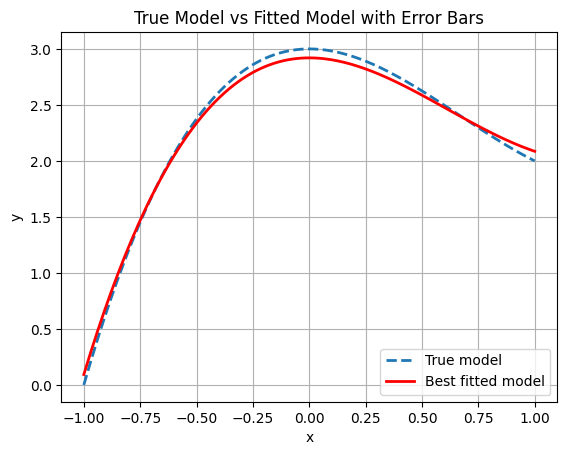
\includegraphics[width=0.48\textwidth]{MSc_Statistics_Research_Report_Template/images/sigma0.5.png} &
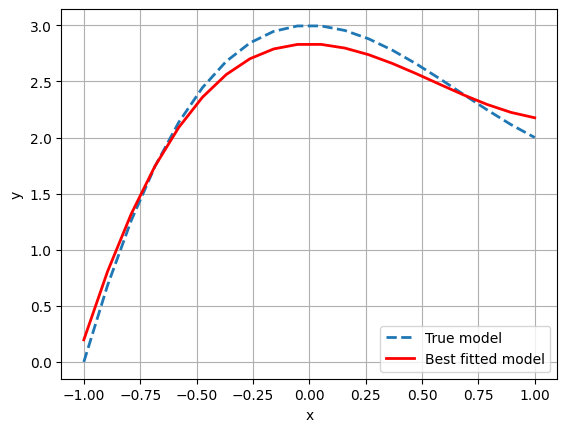
\includegraphics[width=0.48\textwidth]{MSc_Statistics_Research_Report_Template/images/sigma1.0.png} \\
\small (a) $\sigma^2=0.5$ & \small (b) $\sigma^2=1.0$ \\
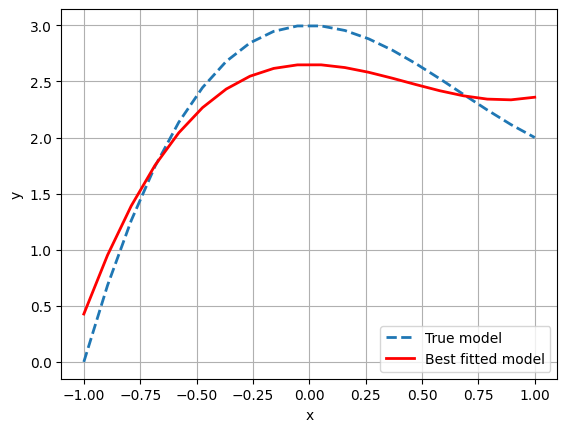
\includegraphics[width=0.48\textwidth]{MSc_Statistics_Research_Report_Template/images/sigma2.0.png} &
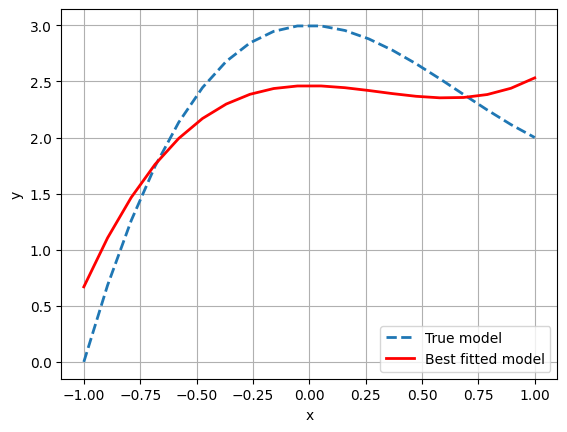
\includegraphics[width=0.48\textwidth]{MSc_Statistics_Research_Report_Template/images/sigma3.0.png} \\
\small (c) $\sigma^2=2.0$ & \small (d) $\sigma^2=3.0$
\end{tabular}
\caption{Comparison of the true model and best fitted model under different noise variances.}
\label{fig:true_vs_fitted}
\end{figure}







\subsection{Study 2: STLSQ Framework}
\label{subsec:STLSQ}
This subsection investigates the performance of the STLSQ method for polynomial regression with additive noise in the response variable. In particular, we study a univariate regression problem where the true underlying model is the sixth-order polynomial $y = 3 - 2x + 0.5x^3 + x^5,$
corrupted by additive Gaussian noise $\varepsilon_i \sim \mathcal{N}(0, 0.05^2)$. We generate $n=1000$ evenly spaced design points over the interval $[-1,1]$ and construct the corresponding polynomial feature library up to degree five. 

To evaluate the effectiveness of sparse regression, we compare two approaches for selecting the sparsity threshold $\lambda$. \begin{itemize}
\item Method 1: The sparsity threshold $\lambda$ is selected by first performing OLS regression and identifying the smallest non-zero coefficient in magnitude. We then set:
$\lambda = 0.9 \times \min(|\text{non-zero OLS coefficients}|).$

The smallest non-zero coefficient from the OLS fit can be regarded as the weakest yet still relevant feature. If the threshold were set exactly equal to this value, the corresponding coefficient would be eliminated during sparsification, potentially removing a meaningful feature. Multiplying by 0.9 lowers the threshold slightly below this boundary, thereby preserving the smallest coefficient while discarding smaller noise-dominated terms. This scaling factor mitigates the risk of erroneous elimination caused by numerical rounding or fluctuations in noisy data.
\item Method 2: Grid-search with BIC: 
We perform a grid search over logarithmically spaced values of $\lambda$ with the optimal value determined by minimising the BIC:
\begin{equation}
    \mathrm{BIC} = n \ln\!\left(\frac{\mathrm{RSS}}{n}\right) + k \ln(n),
\end{equation}
where $\mathrm{RSS}_{\text{STLSQ}}
= \sum_{i=1}^{n}\bigl(y_i - \mathbf{\Phi}(\boldsymbol{x_i})^\top \widehat{\boldsymbol{w}}\bigr)^2$ denotes the residual sum of squares, $k$ is the number of nonzero coefficients. 

The resulting sparse coefficients from both methods are then compared against the truth polynomial coefficients.
\end{itemize}




\begin{table}[htbp]
\centering
\caption{Comparison of STLSQ sparse regression results under different Gaussian noise levels $\sigma$.}
\label{tab:stlsq_noise}
\scriptsize
\begin{tabular}{c p{6cm} p{6cm}}
\toprule
$\sigma$ & Method 1 (OLS$\times 0.9$) & Method 2 (BIC) \\
\midrule
0.05 & $\lambda=0.0027$\newline coeffs = (2.99, -2.00, 0.00, 0.51, 0.02, 0.99) 
      & $\lambda=0.0032$\newline coeffs = (2.99, -2.00, 0, 0.51, 0.02, 0.99) \\
\midrule
0.10 & $\lambda=0.0054$\newline coeffs = (2.99, -2.01, 0.01, 0.53, 0.03, 0.98) 
      & $\lambda=0.0065$\newline coeffs = (2.99, -2.01, 0, 0.53, 0.04, 0.98) \\
\midrule
0.30 & $\lambda=0.0162$\newline coeffs = (2.96, -2.03, 0.02, 0.58, 0.09, 0.94) 
      & $\lambda=0.0187$\newline coeffs = (2.96, -2.03, 0, 0.58, 0.11, 0.94) \\
\midrule
0.50 & $\lambda=0.0270$\newline coeffs = (2.94, -2.05, 0.03, 0.64, 0.15, 0.90) 
      & $\lambda=0.7038$\newline coeffs = (2.98, -1.90, 0, 0, 0, 1.45) \\
\bottomrule
\end{tabular}
\end{table}


Table~\ref{tab:stlsq_noise} reports the estimated coefficients, and Figure~\ref{fig:stlsq} shows the fitted curves against noisy data. From both the coefficients and the visual comparison, the BIC-based rule generally produces fits closer to the true polynomial than the OLS-based rule. However, under noise contamination, neither method is able to perfectly recover the true sparse structure. As the noise variance increases, the quality of the recovered coefficients deteriorates and the fitted curves deviate more substantially from the ground truth. This illustrates that while BIC offers relatively better stability than the OLS-based threshold, both approaches suffer from degraded performance in high-noise regimes. These findings demonstrate that the SINDy framework is highly sensitive to measurement noise, which motivates the development of more robust extensions such as ODR-based approaches in the errors-in-variables setting.




\subsection{Study 3: STLSQ\_ODR Framework}
\label{subsec:study2}
This subsection evaluates the performance of the STLSQ\_ODR procedures for the polynomial regression model with added noise in both predictor variables and the response variable. 
Meanwhile, we randomly set a univariate polynomial regression, which is given by $y = 3 - 2x + 0.5x^3 + x^5$ with $x^2$ and $x^4$ set to zero to induce sparsity. 
We add noise to both input and output variables.
\begin{align*}
x_i^{\text{obs}} &= x_i + \varepsilon_x, \quad \varepsilon_x \sim (0, \sigma_x^2), \\
y_i^{\text{obs}} &= y_i + \varepsilon_y, \quad \varepsilon_y \sim (0, \sigma_y^2).
\end{align*}

\begin{figure}
\centering
\begin{minipage}{0.45\textwidth}
    \centering
    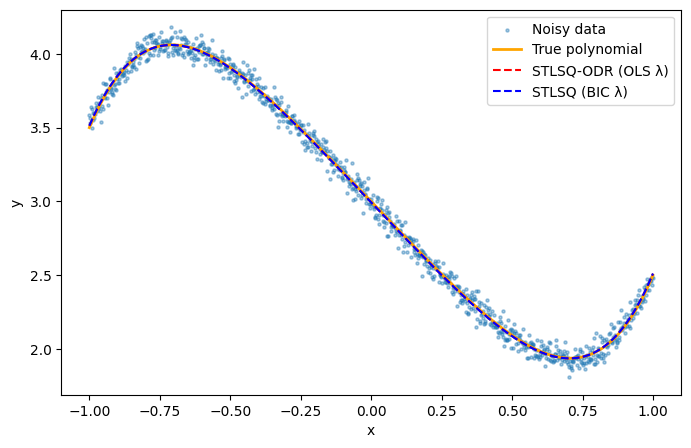
\includegraphics[width=\linewidth]{MSc_Statistics_Research_Report_Template/images/2 0.05.png}
    \subcaption{$\sigma = 0.05$}
\end{minipage}
\begin{minipage}{0.45\textwidth}
    \centering
    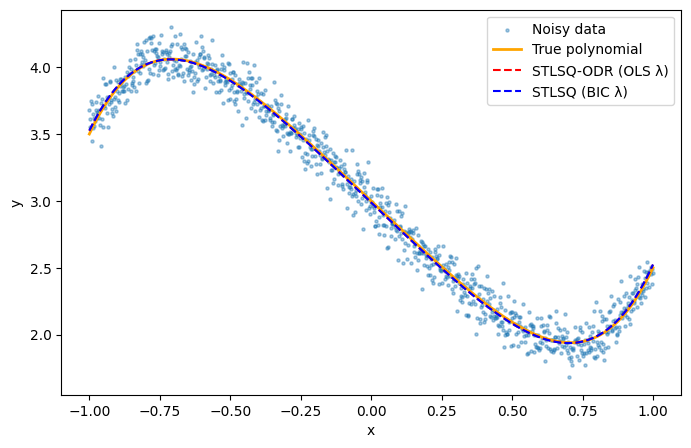
\includegraphics[width=\linewidth]{MSc_Statistics_Research_Report_Template/images/2 0.1.png}
    \subcaption{$\sigma = 0.1$}
\end{minipage}
\begin{minipage}{0.45\textwidth}
    \centering
    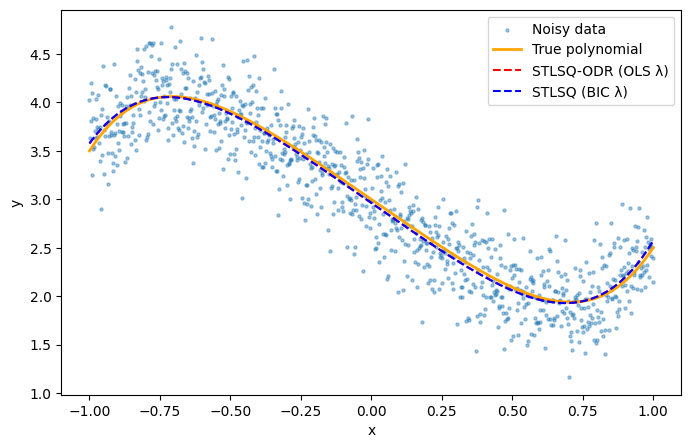
\includegraphics[width=\linewidth]{MSc_Statistics_Research_Report_Template/images/2 0.3.png} 
    \subcaption{$\sigma = 0.3$}
\end{minipage}
\begin{minipage}{0.45\textwidth}
    \centering
    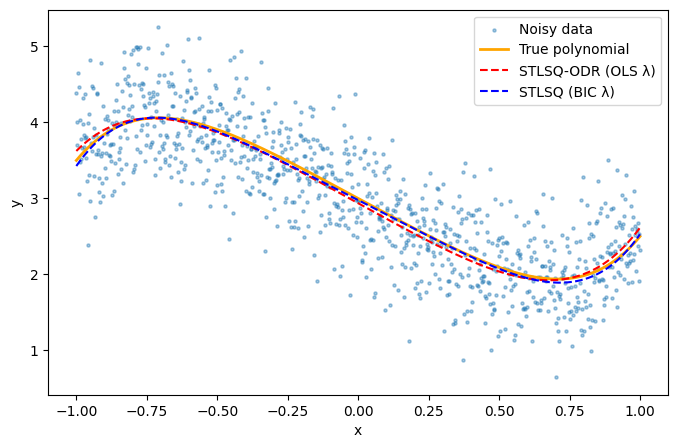
\includegraphics[width=\linewidth]{MSc_Statistics_Research_Report_Template/images/2 0.5.png}
    \subcaption{$\sigma = 0.05$}
\end{minipage}
\caption{Comparison of STLSQ sparse regression results under different Gaussian noise variances $\sigma$.}
\label{fig:stlsq}
\end{figure}

\begin{itemize}
\item Case 1: We add independent Gaussian noise to both input and output variables.

\item Case 2: We add independent Student-t noise to both input and output variables.

\item Case 3: We add correlated Gaussian noise to both input and output variables.

\item Case 4: We add correlated Student-t noise to both input and output variables.
\end{itemize}
we sample $n=1000$ input points uniformly over the domain $[−1,1]$.

We also compare BIC-base and OLS-base to choose different thresholds $\lambda$ in STLSQ\_ODR model selection.
With additive adjustments $\boldsymbol{\delta}_i\in\mathbb{R}^m$ to the predictors and a weighting ratio $d = \sigma_y^{2}/\sigma_x^{2}$,
ODR fits $(w,\{\boldsymbol{\delta}_i\})$ by minimizing
\[
J(\boldsymbol{w},\{\boldsymbol{\delta}_i\}) \;=\; \sum_{i=1}^{n}
\Bigl( y_i - \mathbf{\Phi}(\boldsymbol{x}_i+\boldsymbol{\delta}_i)^\top \boldsymbol{w} \Bigr)^2
\;+\; d\,\|\boldsymbol{\delta}_i\|^2 .
\]



Let $(\widehat{w},\{\widehat{\delta}_i\})$ be the minimizer. We then define the
profiled orthogonal residual sum as
\[
\mathrm{RSS}_{\text{ODR}}
= \sum_{i=1}^{n}
\Bigl( y_i - \mathbf{\Phi}(\boldsymbol{x}_i+\widehat{\boldsymbol{\delta}}_i)^\top \widehat{\boldsymbol{w}} \Bigr)^2
\;+\; d\,\|\widehat{\boldsymbol{\delta}}_i\|^2 ,
\]
and compute
\[
\mathrm{BIC}_{\text{ODR}}
= n\ln\!\Bigl(\tfrac{\mathrm{RSS}_{\text{ODR}}}{n}\Bigr) + k\ln n.
\]
Here $k$ counts the nonzero coefficients in $\widehat{\boldsymbol{w}}$. This replaces the vertical RSS with the profiled orthogonal distance appropriate for EIV.




\paragraph{Case 1}

\begin{table}
\centering
\caption{Comparison of STLSQ-ODR sparse regression results under different Gaussian noise variances $(\sigma_x^2, \sigma_y^2)$.}
\label{tab:sparse_noise}
\scriptsize
\begin{tabular}{c p{6cm} p{6cm}}
\toprule
$(\sigma_x^2, \sigma_y^2)$ & Method 1 (BIC) & Method 2 (OLS$\times 0.9$) \\
\midrule
(0.01, 0.01) & $\lambda=0.0082$\newline coeffs = (3.00, -2.00, 0, 0.50, 0, 1.00) 
             & $\lambda=0.0143$\newline coeffs = (3.00, -2.00 0, 0.50, 0, 1.00) \\
\midrule
(0.05, 0.05) & $\lambda=0.0335$\newline coeffs = (2.99, -2.002, 0, 0.50, 0, 0.96) 
             & $\lambda=0.0272$\newline coeffs = (2.98, -2.00, 0.07, 0.54, -0.07, 0.92) \\
\midrule
(0.1, 0.1)   & $\lambda=0.0677$\newline coeffs = (2.996, -2.00, 0, 0.53, 0, 0.86) 
             & $\lambda=0.0195$\newline coeffs = (2.97, -2.03, 0.12, 0.72, -0.13, 0.67) \\
\midrule
(0.2, 0.2)   & $\lambda=0.0602$\newline coeffs = (2.98, -2.42, 0, 2.21, 0, -0.61) 
             & $\lambda=0.0121$\newline coeffs = (2.95, -2.32, 0.13, 2.06, -0.08, -0.58) \\
\midrule
(0.3, 0.3)   & $\lambda=0.0335$\newline coeffs = (2.98, -2.52, 0, 2.13, 0, -0.50) 
             & $\lambda=0.0053$\newline coeffs = (2.96, -2.59, 0.06, 2.58, 0, -0.77) \\
\midrule
(0.4, 0.4)   & $\lambda=0.4954$\newline coeffs = (2.99, -1.12, 0, 0, 0, 0) 
             & $\lambda=0.0242$\newline coeffs = (2.99, -3.00, 0, 2.90, 0, -0.71) \\
\bottomrule
\end{tabular}
\end{table}

\begin{figure}
\centering
\begin{minipage}{0.45\textwidth}
    \centering
    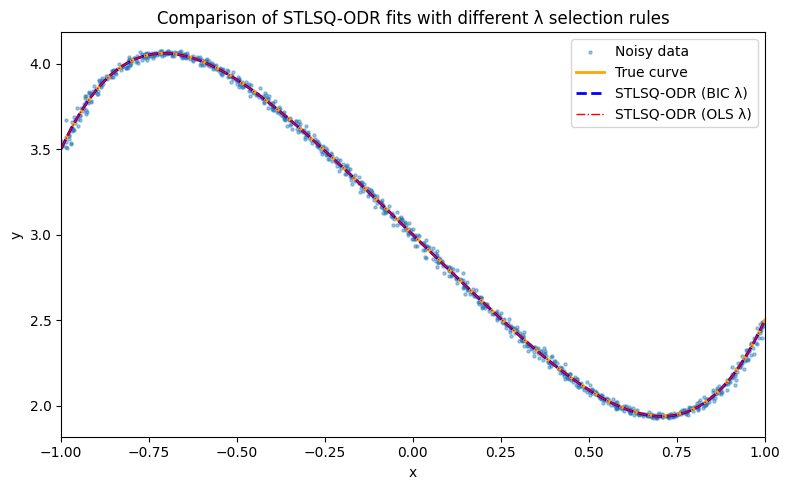
\includegraphics[width=\linewidth]{MSc_Statistics_Research_Report_Template/images/0.01,0.01.png}
    \subcaption{$\sigma_x^2 = 0.01, \; \sigma_y^2 = 0.01$}
\end{minipage}
\begin{minipage}{0.45\textwidth}
    \centering
    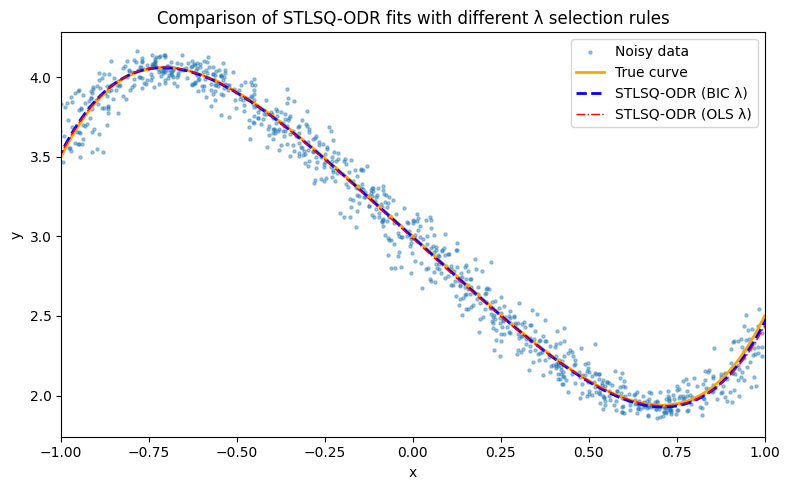
\includegraphics[width=\linewidth]{MSc_Statistics_Research_Report_Template/images/0.05, 0.05.png}
    \subcaption{$\sigma_x^2 = 0.05, \; \sigma_y^2 = 0.05$}
\end{minipage}

\begin{minipage}{0.45\textwidth}
    \centering
    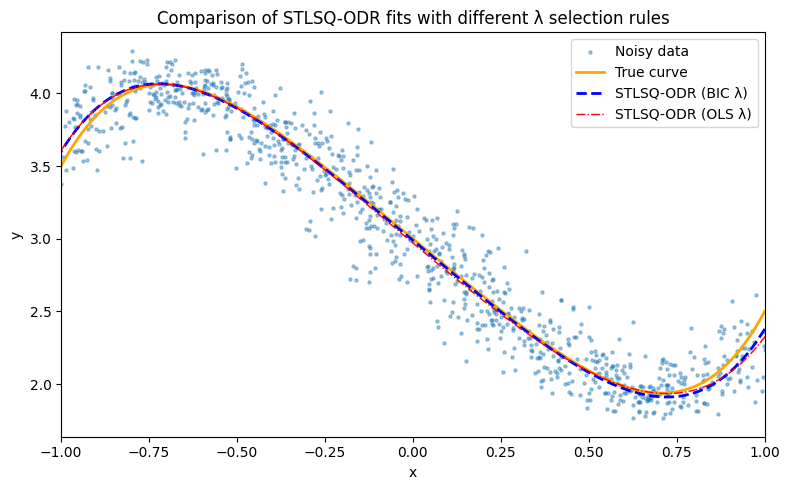
\includegraphics[width=\linewidth]{MSc_Statistics_Research_Report_Template/images/0.1, 0.1.png}
    \subcaption{$\sigma_x^2 = 0.1, \; \sigma_y^2 = 0.1$}
\end{minipage}
\begin{minipage}{0.45\textwidth}
    \centering
    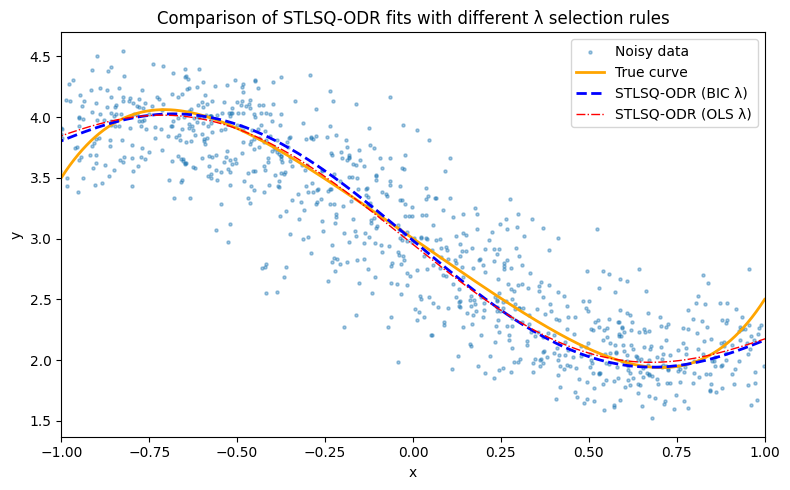
\includegraphics[width=\linewidth]{MSc_Statistics_Research_Report_Template/images/0.2, 0.2.png}
    \subcaption{$\sigma_x^2 = 0.2, \; \sigma_y^2 = 0.2$}
\end{minipage}

\begin{minipage}{0.45\textwidth}
    \centering
    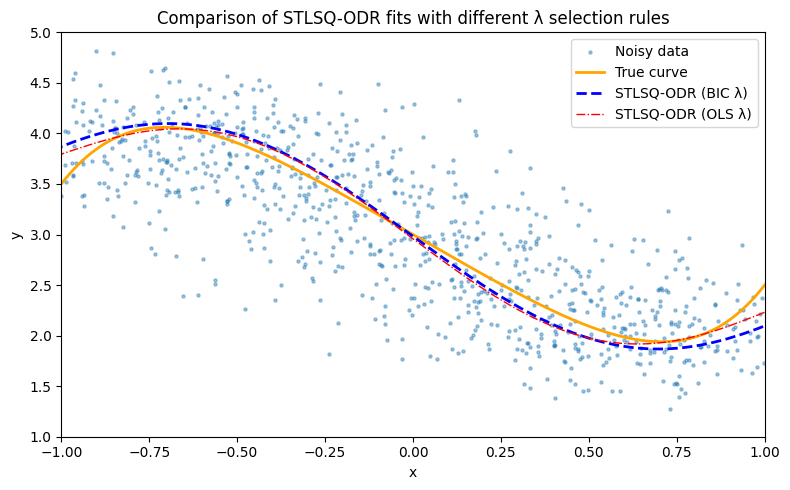
\includegraphics[width=\linewidth]{MSc_Statistics_Research_Report_Template/images/0.3,0.3.png}
    \subcaption{$\sigma_x^2 = 0.3, \; \sigma_y^2 = 0.3$}
\end{minipage}
\begin{minipage}{0.45\textwidth}
    \centering
    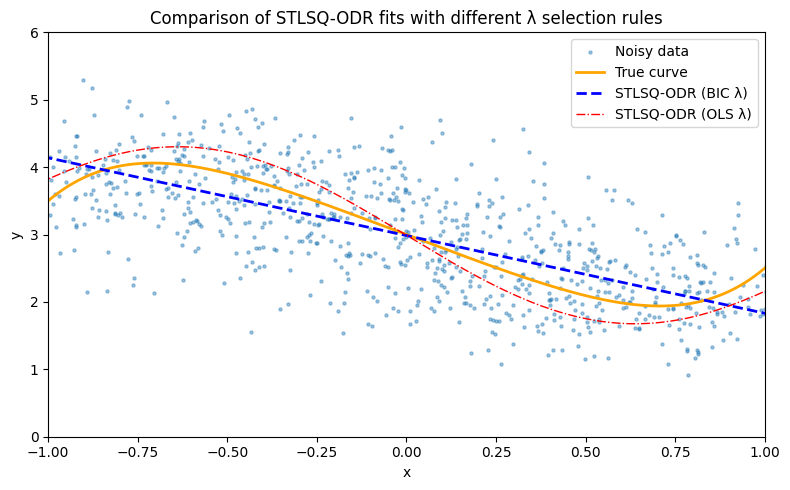
\includegraphics[width=\linewidth]{MSc_Statistics_Research_Report_Template/images/0.4,0.4.png}
    \subcaption{$\sigma_x^2 = 0.4, \; \sigma_y^2 = 0.4$}
\end{minipage}
\caption{Comparison of STLSQ-ODR sparse regression results under different Gaussian noise variances $(\sigma_x^2, \sigma_y^2)$}
\label{fig:stlsq_odr_g}
\end{figure}


Table \ref{tab:sparse_noise} and Figure \ref{fig:stlsq_odr_g} illustrate the performance of STLSQ-ODR under varying Gaussian noise variances $(\sigma_x^2,\sigma_y^2)$. When the noise is small ($\sigma_x^2=\sigma_y^2=0.01$), both BIC-based and OLS-based $\lambda$ selection rules successfully recover the correct sparse polynomial structure. However, once the noise variance exceeds approximately $0.05$, the OLS-based rule fails to shrink irrelevant coefficients to zero, while the BIC-based method continues to make correct model selections as long as the noise remains moderate.



When the noise becomes large ($\sigma^2 \geq 4$), both methods fail to identify the true model structure and produce biased coefficient estimates, indicating the breakdown of sparse recovery under high noise. In particular, the BIC-based method tends to oversimplify the model by shrinking towards an incorrect linear form.



\paragraph{Case 2}

Under Student-$t$ noise, the performance of STLSQ-ODR demonstrates similar patterns as in the Gaussian case, but with more pronounced instability due to heavy-tailed perturbations. As shown in Table \ref{tab:sparse_noise2} and Figure \ref{fig:stlsq_odr_t}, when the noise variance is small ($\sigma^2 \leq 0.01$), both the BIC-based and OLS-based $\lambda$ selection methods successfully recover the true polynomial structure with accurate coefficient estimates. However, once the noise level increases to $\sigma^2 \geq 0.05$, the OLS-based method already fails to shrink irrelevant coefficients to zero, while the BIC-based method remains relatively robust and continues to produce correct model selection. 

\begin{table}[htbp]
\centering
\caption{Comparison of STLSQ-ODR sparse regression results under different Student-t noise variances $(\sigma_x^2, \sigma_y^2)$.}
\label{tab:sparse_noise2}
\scriptsize
\begin{tabular}{c p{6cm} p{6cm}}
\toprule
$(\sigma_x^2, \sigma_y^2)$ & Method 1 (BIC) & Method 2 (OLS$\times 0.9$) \\
\midrule
(0.01, 0.01) & $\lambda=0.0029$\newline coeffs = (3.00, -2.00, 0, 0.53, 0, 0.97) 
             & $\lambda=0.0047$\newline coeffs = (3.00, -2.00, 0, 0.53, 0, 0.96) \\
\midrule
(0.05, 0.05) & $\lambda=0.3486$\newline coeffs = (3.01, -2.23, 0, 1.55, 0, 0) 
             & $\lambda=0.0280$\newline coeffs = (3.01, -2.05, 0, 0.82, 0, 0.62) \\
\midrule
(0.1, 0.1)   & $\lambda=0.1081$\newline coeffs = (3.01, -2.38, 0, 2.00, 0, -0.38) 
             & $\lambda=0.0754$\newline coeffs = (3.03, -2.36, -0.20, 2.11, 0.21, -0.52) \\
\midrule
(0.2, 0.2)   & $\lambda=0.4406$\newline coeffs = (3.03, -1.14, 0, 0, 0, 0) 
             & $\lambda=0.0206$\newline coeffs = (3.08, -2.08, -0.31, 1.22, 0.17, -0.14) \\
\bottomrule
\end{tabular}
\end{table}

When the noise becomes moderate ($\sigma^2 = 0.1$ or $0.2$), both methods exhibit degraded performance, with the BIC-based method tending to oversimplify the model by collapsing to an incorrect linear form, whereas the OLS-based method produces biased estimates with spurious nonzero terms. This highlights the additional difficulty of sparse recovery under heavy-tailed noise, where extreme perturbations significantly affect stability and reliability of coefficient estimation.

\begin{figure}[htbp]
\centering
\begin{minipage}{0.45\textwidth}
    \centering
    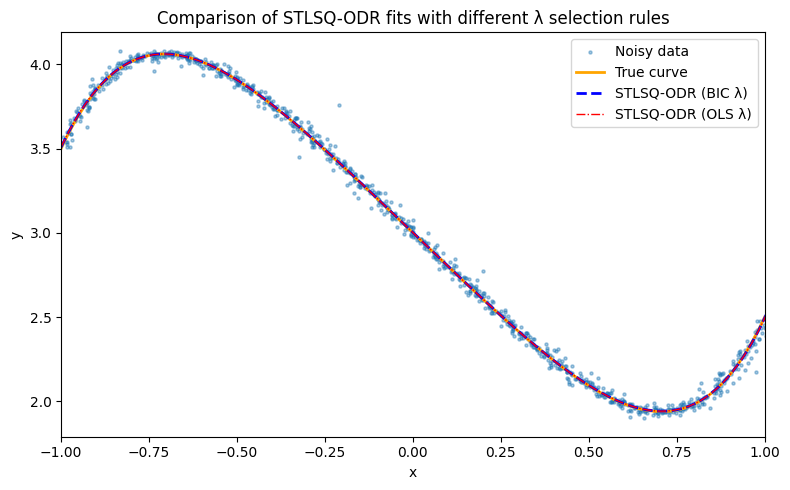
\includegraphics[width=\linewidth]{MSc_Statistics_Research_Report_Template/images/t10.01,0.01.png}
    \subcaption{$\sigma_x^2 = 0.01, \; \sigma_y^2 = 0.01$}
\end{minipage}
\begin{minipage}{0.45\textwidth}
    \centering
    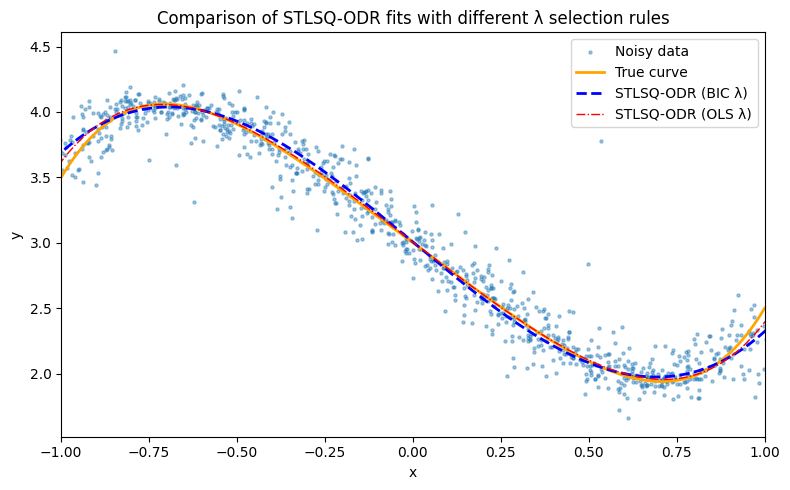
\includegraphics[width=\linewidth]{MSc_Statistics_Research_Report_Template/images/t 0.05,0.05.png}
    \subcaption{$\sigma_x^2 = 0.05, \; \sigma_y^2 = 0.05$}
\end{minipage}

\begin{minipage}{0.45\textwidth}
    \centering
    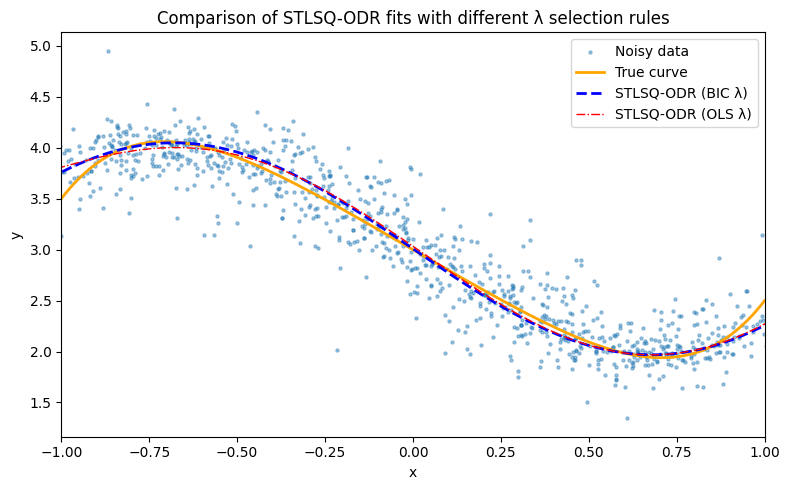
\includegraphics[width=\linewidth]{MSc_Statistics_Research_Report_Template/images/t0.1,0.1.png} 
    \subcaption{$\sigma_x^2 = 0.1, \; \sigma_y^2 = 0.1$}
\end{minipage}
\begin{minipage}{0.45\textwidth}
    \centering
    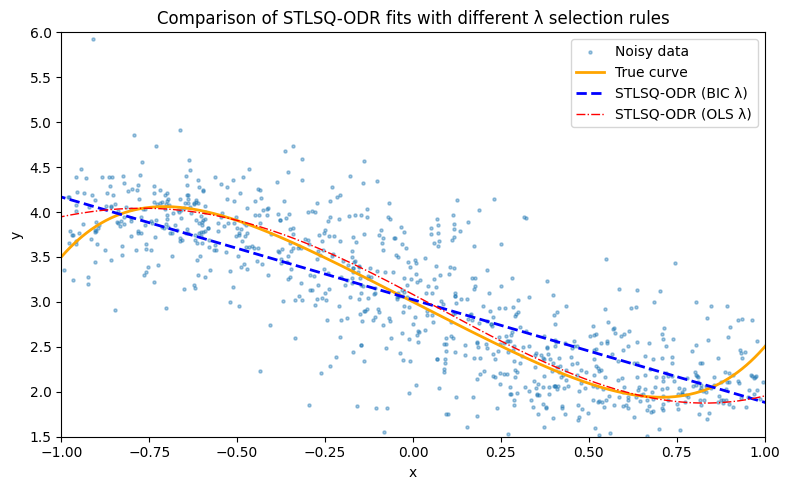
\includegraphics[width=\linewidth]{MSc_Statistics_Research_Report_Template/images/t0.2,0.2.png}
    \subcaption{$\sigma_x^2 = 0.2, \; \sigma_y^2 = 0.2$}
\end{minipage}

\caption{Comparison of STLSQ-ODR sparse regression results under different Student-t noise variances $(\sigma_x^2, \sigma_y^2)$.}
\label{fig:stlsq_odr_t}
\end{figure}

\paragraph{Case 3}

To further examine the effect of correlated Gaussian noise, we consider the case where both predictor and response variables are perturbed with correlated Gaussian errors of equal variance $\sigma_x^2 = \sigma_y^2$, under varying correlation levels $\rho \in [0.1, 1.0]$. As shown in Table \ref{tab:cor}, the sparse recovery results demonstrate that the BIC-based thresholding method generally outperforms the OLS-based method. In particular, for low to moderate noise levels ($\sigma_x = \sigma_y \leq 0.05$), the BIC-based method consistently recovers the correct polynomial structure with accurate coefficient estimates, whereas the OLS-based method tends to include additional small spurious terms, reflecting reduced stability under correlated noise.
As the noise variance increases, this performance gap becomes more evident. For example, at $\sigma_x = \sigma_y = 0.05$ with $\rho=1.0$, the OLS-based method admits extra nonzero terms, while the BIC-based method still maintains sparsity and accurate recovery. This highlights the stronger robustness of the BIC-based criterion in balancing model fit and complexity under correlated perturbations.

However, when the noise level becomes large ($\sigma_x = \sigma_y = 0.07, \rho=1.0$), even the BIC-based method fails to correctly identify the true model. This breakdown indicates that under high-variance correlated Gaussian noise, the signal-to-noise ratio becomes too low for reliable sparse recovery.

\begin{table}[htbp]
\centering
\caption{Comparison of sparse regression results under different correlation levels $\rho$ and Gaussian noise scales $\sigma_x$, $\sigma_y$.}
\label{tab:cor}
\scriptsize
\begin{tabular}{c c p{6cm} p{6cm}}
\toprule
$\sigma_x,\sigma_y$ & $\rho$ & Method 1 (BIC) & Method 2 (OLS$\times 0.9$) \\
\midrule
0.01 & 0.1 
& $\lambda=0.0058$\newline coeffs = (3.00, -2.01, 0, 0.53, 0, 0.97) 
& $\lambda=0.0041$\newline coeffs = (3.00, -2.01, 0.01, 0.53, -0.01, 0.97) \\
\midrule
0.01 & 1.0 
& $\lambda=0.0092$\newline coeffs = (3.00, -2.01, 0, 0.52, 0, 0.98) 
& $\lambda=0.0065$\newline coeffs = (3.00, -2.01, 0.02, 0.52, -0.02, 0.98) \\
\midrule
0.05 & 0.1 
& $\lambda=0.0236$\newline coeffs = (3.00, -2.03, 0, 0.57, 0, 0.93) 
& $\lambda=0.0226$\newline coeffs = (3.00, -2.03, 0.04, 0.56, -0.05, 0.94) \\
\midrule
0.05 & 1.0 
& $\lambda=0.0298$\newline coeffs = (3.00, -2.07, 0, 0.68, 0, 0.88) 
& $\lambda=0.0232$\newline coeffs = (2.99, -2.07, 0.06, 0.68, -0.06, 0.89) \\
\midrule
0.07 & 1.0 
& $\lambda=0.3919$\newline coeffs = (3.00, -2.34, 0, 1.71, 0, 0) 
& $\lambda=0.0362$\newline coeffs = (2.99, -2.12, 0.08, 0.77, -0.09, 0.86) \\
\bottomrule
\end{tabular}
\end{table}




\paragraph{Case 4}

We consider the case where both input and output variables are perturbed with correlated Student-t noise of equal variance $\sigma_x^2 = \sigma_y^2 = 0.02$. As shown in Table \ref{tab:sparse_rho}, the sparse recovery results remain relatively stable across different correlation levels $\rho \in [0.1, 1.0]$. Both BIC-based and OLS-based $\lambda$ selection methods consistently identify the correct polynomial structure, with coefficient estimates close to the ground truth. 

However, a gradual increase in correlation slightly reduces the sparsity and stability of the OLS-based method, leading to the inclusion of small spurious terms when $\rho=1.0$. In contrast, the BIC-based method remains more conservative, maintaining exact sparsity throughout all correlation levels. These findings suggest that while correlated noise does not fundamentally impair sparse recovery at moderate noise levels, it can introduce additional estimation bias in OLS-based selection, whereas BIC-based selection exhibits stronger robustness.

\begin{table}[htbp]
\centering
\caption{Comparison of sparse regression results under different correlation levels $\rho$ when Student-t noise scales are $\sigma_x=0.02$ and $\sigma_y=0.02$. }
\label{tab:sparse_rho}
\scriptsize
\begin{tabular}{c p{6cm} p{6cm}}
\toprule
$\rho$ & Method 1 (BIC) & Method 2 (OLS$\times 0.9$) \\
\midrule
0.1 & $\lambda=0.0018$\newline coeffs = (3.00, -2.04, 0, 0.68, 0, 0.81) 
    & $\lambda=0.0542$\newline coeffs = (3.00, -2.03, 0, 0.62, 0, 0.88) \\
\midrule
0.5 & $\lambda=0.0013$\newline coeffs = (3.00, -2.06, 0, 0.73, 0, 0.78) 
    & $\lambda=0.0371$\newline coeffs = (3.00, -2.04, 0, 0.65, 0, 0.87) \\
\midrule
0.8 & $\lambda=0.0032$\newline coeffs = (3.00, -2.06, 0, 0.75, 0, 0.77) 
    & $\lambda=0.0313$\newline coeffs = (3.00, -2.051, 0, 0.65, 0, 0.88) \\
\midrule
1.0 & $\lambda=0.0131$\newline coeffs = (3.00, -2.06, 0, 0.74, 0, 0.80) 
    & $\lambda=0.0262$\newline coeffs = (3.00, -2.04, 0.05, 0.59, -0.06, 0.94) \\
\bottomrule
\end{tabular}
\end{table}



















